\chapter{Preliminaries}\label{chap:preliminaries}

This chapter introduces the essential concepts and terminology referenced in the rest of the thesis, providing the necessary background to understand the arguments developed in subsequent chapters.

\section{Extensible Markup Language (XML)}\label{sec:xml}

\gls{xml} is a markup language and file format designed to store structured data.
It is regarded as an \emph{application} (a subset) of \gls{sgml}, an earlier markup language~\cite[Sec. 1.1]{xml11}.

It was designed to facilitate the straightforward transfer of documents over the Internet~\cite[Sec. 1.1]{xml11}. The format features a human-readable structure, with relatively little effort required to implement \gls{xml} parsers~\cite[Sec. 1.1]{xml11}.

An \gls{xml} document is made up of \emph{entities}, which form an \emph{entity tree}~\cite[Sec. 2]{xml11}.

In the rest of this section, we will cover the most important concepts found in \gls{xml}.

\subsection{CDATA}

CDATA sections behave similarly to text. They are parsed, but their contents are interpreted verbatim. This makes it possible to include text in \gls{xml} that would otherwise be interpreted as markup (for example, text containing the characters \texttt{<} and \texttt{\&}). A CDATA section is initiated by \texttt{<![CDATA[} and terminated by \texttt{]]>}. 
\begin{samepage}
For instance:
\begin{minted}{xml}
    <![CDATA[We can use < and & here.]]>
\end{minted}
\end{samepage}
\begin{samepage}
CDATA sections can be useful for embedding \gls{css} or JavaScript source code in \gls{svg}:
\begin{minted}{xml}
    <style type="text/css">
    <![CDATA[
        rect {
            color: red;
        }
    ]]>
    </style>
\end{minted}
\end{samepage}

\subsection{Comments}

Comments are strings of text that do not affect the document semantics~\cite[Sec. 2.5]{xml11}. They are typically used for documentation purposes. A comment starts with \texttt{<!-{}-} and ends with \texttt{-{}->}~\cite[Sec. 2.5]{xml11}. Comments cannot be nested and may be discarded by the parser~\cite[Sec. 2.5]{xml11}. As an example, consider the following \gls{xml} comment:
\begin{minted}{xml}
    <!-- This is a comment. -->
\end{minted}

\subsection{Elements}

Elements are perhaps the most essential building blocks of \gls{xml}. An element is characterized by its name, which specifies its type~\cite[Sec. 3]{xml11}. An element may be \emph{empty}, in which case we call it an \emph{empty element}, or may contain other elements as \emph{children}~\cite[Sec. 3]{xml11}. An element may also optionally contain a set of \emph{attributes}~\cite[Sec. 3]{xml11}. Elements are denoted by \emph{tags}~\cite[Sec. 3]{xml11}. As an example, we provide the following code snippet:
\begin{minted}{xml}
    <g>
        <rect width="10" height="20" />
    </g>
\end{minted}

\subsection{Tags}

\begin{samepage}
Tags encompass elements~\cite[Sec. 3]{xml11}. There are three types of tags~\cite[Sec. 3]{xml11}:
\begin{itemize}
    \item \emph{start-tag}: \xml{<name>},
    \item \emph{end-tag}: \xml{</name>},
    \item \emph{empty-element-tag}: \xml{<name />}.
\end{itemize}
\end{samepage}

\subsection{Attributes}

Attributes are key-value pairs associated with an element~\cite[Sec. 3.3]{xml11}. Each attribute name has a corresponding data type and, optionally, a default value~\cite[Sec. 3.3]{xml11}. Attributes carry the form \xml{name="value"}~\cite[Sec. 3.3]{xml11}.

\section{Scalable Vector Graphics (SVG)}\label{theo:svg}

\gls{svg} is an \gls{xml}-based file format for describing two-dimensional graphics~\cite[Sec. 1.1]{svg11}. Although the typical use of \gls{svg} is to create vector graphics, \gls{svg} documents can also include text and raster images~\cite[Sec.~2]{svg11}. \gls{svg} was designed and is currently maintained by the \gls{w3c}~\cite{svg11, svg2, svg2-draft}. A recent analysis indicates that more than 60~\% of all websites on the Internet use \gls{svg} to store image content, showing its widespread use~\cite{imageformats}.

\gls{svg} is an application of \gls{xml} and, as such, consists of the same entities as described in Section~\ref{sec:xml}.

In \gls{svg}, elements are used to represent graphical objects. The list of elements defined in the \gls{svg} specification~\cite{svg11} includes, but is not limited to:
\begin{itemize}
    \item \texttt{<g>}: used to group other elements,
    \item \texttt{<rect>}, \texttt{<circle>}, \texttt{<ellipse>}, and other: elementary geometric shapes,
    \item \texttt{<svg>}: the root element of every \gls{svg} document,
    \item \texttt{<defs>} and \texttt{<use>}: used to create a single definition of an element (in \texttt{<defs>}) and use it in several places at once (with \texttt{<use>}),
    \item \texttt{<linearGradient>}, \texttt{<radialGradient>}, and \texttt{<pattern>}: used to create complex gradients and patterns that may be subsequently used, for instance, to fill a shape,
    \item \texttt{<path>}: used to define a path,
    \item \texttt{<style>} and \texttt{<script>}: used to embed \gls{css} and JavaScript code in the document,
    \item \texttt{<text>}: used to include textual content,
    \item \texttt{<image>}: used for embedding raster images,
    \item \texttt{<a>}: used to create hyperlinks.
\end{itemize}

Attributes are used to modify the properties of graphical objects\footnote{Additionally, elements may be styled using \gls{css}.}. As an example, consider the following element:
\begin{minted}{xml}
    <rect x="10" y="10" width="50" height="25" />
\end{minted}
This code defines a rectangle positioned at the coordinate $\point{10, 10}$ with a width of 50 units and a height of 25 units.

Multiple versions of \gls{svg} are available. \gls{svg}~1.1~\cite{svg11} remains the latest official \gls{svg} \emph{Recommendation} published by the \gls{w3c}. Although \gls{svg}~2, designed to replace \gls{svg}~1.1, exists as \emph{Candidate Recommendation}~\cite{svg2} and a more recent \emph{Editor's Draft}~\cite{svg2-draft}, neither has reached the full status of Recommendation. This thesis will primarily refer to the \gls{svg}~1.1 specification~\cite{svg11}.

The remainder of this section introduces some of the most fundamental concepts and terminology of \gls{svg}.

\subsection{Attribute types}

In \gls{svg}, attributes can be of several types. Table~\ref{table:attr-types} shows an overview of some of the attribute types defined in the \gls{svg} specification~\cite{svg11}.

\begin{table}[hbtp]
    \centering

    \begin{threeparttable}
        \begin{tabularx}{\linewidth}{p{0.275\linewidth}Xp{0.25\linewidth}}
            \toprule
            \textbf{Name} & \textbf{Description} & \textbf{Example} \\
            \midrule
            \texttt{number} & A real number. May be specified using scientific notation. & 2e+05 \\
            \texttt{integer} & An integer. & 42 \\
            \texttt{length} & A distance measurement. Optionally followed by a unit. & 1cm \\
            \texttt{coordinate} & A position in the coordinate system (single axis). Semantically equivalent to \texttt{length}. & 1.5e-02in \\
            \texttt{angle} & An angle. Optionally followed by a unit. & 45rad \\
            \texttt{points} & A list of vertex coordinates. & 0,0 10,10 \\
            \texttt{color} & A color. May be specified in RGB, HSL, hexadecimal, or named format. & \#00ff00 \\
            \texttt{path-data} & Instructions that define a path. & M 0,0 L 5,1 Z \\
            \texttt{transform-list} & A list of transformations to be applied to an element. & $\operatorname{rotate}(45)\operatorname{scale}(2)$ \\
            \bottomrule
      \end{tabularx}
      
      \caption{An overview of the fundamental attribute types in SVG.}
      \label{table:attr-types}
    \end{threeparttable}
\end{table}

We present some of these types in more detail in subsequent sections.

\subsection{Canvas, viewport, and viewbox}

The \gls{svg} canvas can be thought of as an infinite plane on which the content is drawn~\cite[Sec.~7.1]{svg11}. To represent points in the plane, \gls{svg} uses a Cartesian coordinate system where the ordinate axis is oriented downward, which means the coordinate values increase as we move to the right and down~\cite[Sec.~7.3]{svg11}.

Although the canvas is, in theory, infinite, the content is rendered with respect to a finite rectangular part of the canvas called the \emph{viewport}~\cite[Sec.~7.1]{svg11}. The viewport can be thought of as a \enquote{window} through which we observe the content on the canvas~\cite{brown_svg_viewbox, tutsplus_viewbox_viewport}. If the window is shrunk or enlarged, the apparent size of the content remains unchanged, but the visible portion of the content changes accordingly. The size of the viewport is defined by the attributes \texttt{width} and \texttt{height} on the root \texttt{<svg>} element~\cite[Sec.~7.2]{svg11}.

Furthermore, \gls{svg} defines the concept of \emph{viewbox}. The viewbox can be thought of as a telescope~\cite{tutsplus_viewbox_viewport, aditya_understanding_viewbox}. Similarly to the viewport, the viewbox restricts the portion of the canvas that is visible to the observer. However, unlike the viewport, the viewbox enables panning and zooming, similar to how a telescope may be repositioned to allow one to see a different area of the observed object or magnify a specific section of it~\cite{tutsplus_viewbox_viewport, aditya_understanding_viewbox}. The viewbox is specified by the \texttt{viewBox} attribute on the root \texttt{<svg>} element in the form of a 4-tuple
\[
    \left(x_{min}, y_{min}, w, h\right)\textbf{,}
\]
where $x_{min}$ and $y_{min}$ define the position of the upper left corner of the viewbox, and $w$ and $h$ define the size of the viewbox~\cite[Sec.~7.7]{svg11}.

\subsection{Fill and stroke}

In \gls{svg}, an element may be \emph{filled} and \emph{stroked}~\cite[Sec.~11.1]{svg11}. Filling means applying \emph{paint} (a solid color, gradient, or pattern) to the inside of the element, while stroking refers to painting along the edge of the element~\cite[Sec.~11.1]{svg11}. The difference between stroking and filling is demonstrated in Figure~\ref{fig:stroke-fill}.
\begin{figure}[H]
  \centering
  \begin{subfigure}[b]{0.3\textwidth}
    \centering
    
\begin{tikzpicture}
      \draw[orange, line width=1mm] (0,0) circle (1cm);
    \end{tikzpicture}
    \caption{A circle that is stroked, but not filled.}
  \end{subfigure}
  \hfill
  \begin{subfigure}[b]{0.3\textwidth}
    \centering
    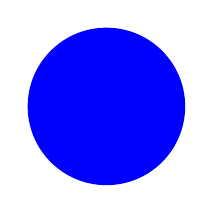
\begin{tikzpicture}
      \path[fill=blue] (0,0) circle (1cm);
    \end{tikzpicture}
    \caption{A circle that is filled, but not stroked.}
  \end{subfigure}
  \hfill
  \begin{subfigure}[b]{0.3\textwidth}
    \centering
    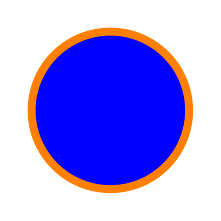
\begin{tikzpicture}
      \draw[orange, line width=1mm, fill=blue] (0,0) circle (1cm);
    \end{tikzpicture}
    \caption{A circle that is both stroked and filled.}
  \end{subfigure}
  \caption{The difference between stroking and filling in SVG.}
  \label{fig:stroke-fill}
\end{figure}

The stroke and fill colors are controlled by the \texttt{stroke} and \texttt{fill} attributes, respectively~\cite[Sec.~11.2]{svg11}. The width (thickness) of the stroke can be set using \texttt{stroke-width}; the default value is the width of one pixel~\cite[Sec.~11.4]{svg11}.

\subsection{Basic shape}

A common and simple \emph{shape} that is predefined for convenience as an element~\cite[Sec.~1.6]{svg11}. The basic shapes are~\cite[Sec.~1.6]{svg11}:
\begin{itemize}
    \item \texttt{<rect>}: a rectangle,
    \item \texttt{<circle>}: a circle,
    \item \texttt{<ellipse>}: an ellipse,
    \item \texttt{<line>}: a line segment,
    \item \texttt{<polyline>}: a series of connected line segments,
    \item \texttt{<polygon>} a series of connected line segments that form a closed shape.
\end{itemize}

\subsection{Shape}

A shape is a \emph{graphics element} that is \enquote{defined by some combination of straight lines and curves}~\cite[Sec.~1.6]{svg11}. Shapes include all \emph{basic shapes} as well as the \texttt{<path>} element~\cite[Sec.~1.6]{svg11}.

\subsection{Graphics element} 

A graphics element in \gls{svg} is any element that causes graphics to be drawn on the canvas~\cite[Sec.~1.6]{svg11}. Graphics elements include all \emph{shapes} as well as the \texttt{<text>} and \texttt{<use>} elements.

\subsection{Paths}

Paths are perhaps the most important building block of \gls{svg}. They allow one to create arbitrarily complex shapes using a simple set of commands. All basic shapes in \gls{svg} can be converted into equivalent path elements \cites[Chap.~10]{svg2}{aleen42_shape_to_path, wichmann_decomposition_basic_svg}.

Paths in \gls{svg} are based on the concept of a virtual \enquote{pen} that moves around the canvas and draws lines and curves to produce the desired shape~\cite[Sec.~8.1]{svg11}. A path is defined by its \emph{path data}: a sequence of elementary drawing operations called \emph{path commands} that describe how the pen moves~\cite[Sec.~8.1]{svg11}. The path commands available in \gls{svg} are listed in Table~\ref{tab:path-commands-theory}~\cite[Sec.~8.3]{svg11}.

\begin{table}[H]
    \centering
    
    \begin{tabular}{c p{4.5cm} p{5cm}}
        \toprule
        \textbf{Character} & \textbf{Name} & \textbf{Description} \\
        \midrule
        m\slash M & moveto & Move the pen without drawing. \\
        z\slash Z & closepath & Close the current subpath by drawing a line segment to the starting point of the subpath. \\ \hline
        l\slash L & lineto & Draw a line segment. \\
        h\slash H & horizontal lineto & Draw a horizontal line segment. \\
        v\slash V & vertical lineto & Draw a vertical line segment. \\ \hline
        q\slash Q & quadratic Bézier curveto & Draw a quadratic Bézier curve. \\
        t\slash T & shorthand\slash smooth quadratic Bézier curveto & Draw a quadratic Bézier curve. \\ \hline
        c\slash C & curveto & Draw a cubic Bézier curve. \\
        s\slash S & shorthand\slash smooth curveto & Draw a cubic Bézier curve.  \\ \hline
        a\slash A & elliptical arc & Draw an elliptical arc. \\
        \bottomrule
    \end{tabular}
    
    \caption{Path commands in SVG.}
    \label{tab:path-commands-theory}
\end{table}

Each path command is expressed by its character and a set of parameters. When the path command character is uppercase, the parameters are interpreted as absolute coordinates~\cite[Sec.~8.3]{svg11}. For example, the path command \texttt{M 10,20} moves the pen to the coordinate $[10, 20]$. On the other hand, path commands with a lowercase command character indicate the use of coordinates that are relative to the current point~\cite[Sec.~8.3]{svg11}. For instance, given a current point $[x, y]$, the command \texttt{m 10,20} moves the pen to $[x + 10, y + 20]$. We use the terms \emph{absolute path command} and \emph{relative path command} to refer to the uppercase and lowercase versions of the commands, respectively.

If a path command is used several times in a row, subsequent command characters may be omitted~\cite[Sec.~8.3.1]{svg11}. As an example, consider the path data \texttt{L 10 20 30 40}, which is semantically equivalent to \texttt{L 10 20 L 30 40}. We use the terms \emph{implicit path command} and \emph{explicit path command} to refer to these two scenarios.

The moveto and closepath commands mark the start and end of a \emph{subpath}, respectively~\cite[Sec.~8.3]{svg11}. A subpath is thus a subset of the path data that forms a continuous curve. A path (potentially discontinuous) may contain more than one subpath, in which case we call it a \emph{compound path}~\cite[Sec.~8.3.1]{svg11}. A subpath (and, by extension, a path) must always start with a moveto command that establishes the initial position of the pen~\cite[Sec.~8.3.2]{svg11}.

Note that closing a path with a closepath command is not necessarily equivalent to \enquote{manually} closing the subpath by drawing a line segment to the starting point of the subpath using the lineto command~\cite[Sec.~8.3.3]{svg11}. In the first case, the starting and ending points will be automatically connected in a way that smoothly connects the stroke around the connection point. However, in the latter case, the ends of the subpath will not be connected smoothly, and the stroke near the end points may appear jagged as a result. We demonstrate this subtle, yet important difference in Figure~\ref{fig:close-path}.

\begin{figure}[H]
    \centering
    \begin{subfigure}[b]{0.45\textwidth}
        \centering
        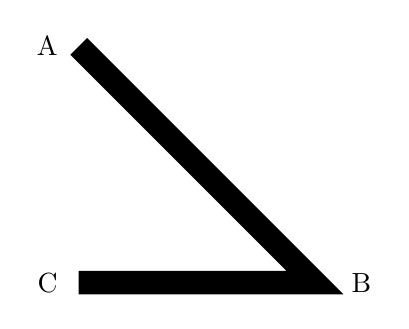
\begin{tikzpicture}[line width=0.3cm]
            \coordinate (A) at (0, 3);
            \coordinate (B) at (3, 0);
            \coordinate (C) at (0, 0);

            \node[left] at (A) {A};
            \node[right, xshift=0.2cm] at (B) {B};
            \node[left] at (C) {C};

            \draw (A) -- (B) -- (C);
        \end{tikzpicture}
        \caption{A subpath closed using the closepath command.}
        \label{fig:close-path-correct}
    \end{subfigure}
    \hfill
    \begin{subfigure}[b]{0.45\textwidth}
        \centering
        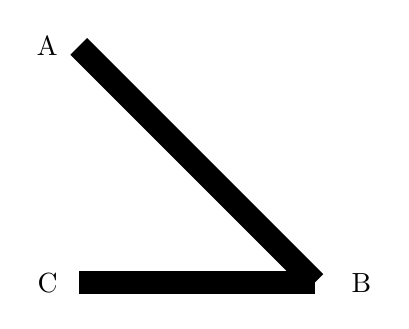
\begin{tikzpicture}[line width=0.3cm]
            \coordinate (A) at (0, 3);
            \coordinate (B) at (3, 0);
            \coordinate (C) at (0, 0);

            \draw (A) -- (B);
            \draw (B) -- (C);

            \node[left] at (A) {A};
            \node[right, xshift=0.2cm] at (B) {B};
            \node[left] at (C) {C};
        \end{tikzpicture}
        \caption{A subpath closed using the lineto command.}
        \label{fig:close-path-incorrect}
    \end{subfigure}
    \caption{A comparison between closing a path using the closepath and lineto commands. Notice the difference in the stroke near point B.}
    \label{fig:close-path}
\end{figure}

We refer to the commands \textbf{H}, \textbf{V}, \textbf{S}, and \textbf{T} as \emph{shorthand commands}. Shorthand commands provide functionality identical to their regular counterparts while requiring fewer parameters~\cite[Sec.~8.3]{svg11}. The values of the missing parameters are inferred from the context\footnote{The method employed varies based on the specific command utilized; in our thesis, we will not go into the specifics of this inference process. See~\cite[Sec.~8.3]{svg11} for more details.}~\cite[Sec.~8.3.2]{svg11}.

A path is specified using the \texttt{<path>} element, with path data defined by the \texttt{d} attribute~\cite[Sec.~8.2]{svg11}. As an example, consider the following element:
\begin{minted}{xml}
    <path d="M0,0 H10 Q 15,7.5 10,10 Z" />
\end{minted}
This path element
\begin{itemize}
    \item starts a new subpath at the coordinate $\point{0, 0}$,
    \item draws a horizontal line segment to $\point{10, 0}$,
    \item draws a quadratic Bézier curve to $\point{10, 10}$ with a control point at $\point{15, 7.5}$,
    \item closes the subpath by drawing a straight line back to $\point{0, 0}$.
\end{itemize}
The visual appearance of this path is shown in Figure~\ref{fig:example-path}.

\begin{figure}[H]
    \centering
    \begin{tikzpicture}[ultra thick, scale=10, yscale=-1]
        \draw svg "M0,0 H10 Q 15,7.5 10,10 Z";
    \end{tikzpicture}
    \caption{A path defined by the path data \texttt{M0,0 H10 Q 15,7.5 10,10 Z}.}
    \label{fig:example-path}
\end{figure}

Formally, we can think of paths as \emph{parametric curves}\footnote{In a strict sense, only \emph{subpaths} can be represented as parametric curves because parametric curves must be continuous. However, we can bypass this limitation by assuming that all paths are made up of exactly one subpath.}. A parametric curve is a continuous function
\[
    \gamma\colon\interval[scaled]{0}{1}\to\mathbb{R}^2
\]
that maps the values of a parameter $t$ to points in $\mathbb{R}^2$. We call the points $\gamma(0)$ and $\gamma(1)$ the \emph{starting} and \emph{ending} points of the curve, respectively. If $\gamma(0) = \gamma(1)$, we say that the curve is \emph{closed}. If a curve is not closed, it is said to be \emph{open}.

\subsection{Transformations}\label{theo:transformations}

In \gls{svg}, elements can be transformed using arbitrary affine transformations~\cite[Sec.~7]{svg11}.

\begin{definition}[Affine transformation]
    An affine transformation is a mapping of the form
    \[
        T(x) = Ax + \vec{b}\text{,}
    \]
    where
    \[
        A =
        \begin{pmatrix}
            a & c \\
            b & d
        \end{pmatrix}
    \]
    is the matrix of a linear transformation and
    \[
        \vec{b} =
        \begin{pmatrix}
            e \\
            f
        \end{pmatrix}
    \]
    is a translation vector.
\end{definition}

Compositions of linear transformations can be conveniently represented using matrix multiplication. However, as translation is non-linear, we cannot use this approach for affine transformations~\cite[Sec.~1.2.1]{salomon2006transformations}. To overcome this limitation, we can represent affine transformations using an augmented matrix in \emph{homogeneous coordinates}~\cite{salomon2006transformations}:
\[
    H =
    \begin{pmatrix}
        a & c & e \\
        b & d & f \\
        0 & 0 & 1
    \end{pmatrix}
    \text{.}
\]
The composition of affine transformations $T_1,T_2,\ldots,T_n$ given by the matrices $H_1,H_2,\ldots,H_n$ in homogeneous coordinates is then simply obtained by post-multiplication of the corresponding transformation matrices:
\[
    T_n \circ T_{n-1} \circ \ldots \circ T_1 = \prod_{i = 1}^n{H_i}\text{.}
\]
Given a point $\point{x, y}$, the transformed point $\point{x', y'}$ is obtained using the following~\cites[Sec.~7.4]{svg11}[Sec.~1.2.1]{salomon2006transformations}:
\[
    \begin{bmatrix}
        x' \\
        y' \\
        1
    \end{bmatrix}
    =
    \begin{pmatrix}
        a & c & e \\
        b & d & f \\
        0 & 0 & 1
    \end{pmatrix}
    \cdot
    \begin{bmatrix}
        x \\
        y \\
        1
    \end{bmatrix}
    \text{.}
\]

Each \gls{svg} element may have an associated \emph{transformation list} specified by the \texttt{transform} attribute~\cite{svg11, svg2}. The transformation list contains a sequence of transformations that are applied to the element in the order of left-to-right~\cite[Sec.~7.4]{svg11}. The transformation may be specified as an affine transformation matrix:
\[
    \operatorname{matrix}(a, b, c, d, e, f)\text{,}
\]
or using one of the predefined \emph{transformation functions}; they are~\cite[Sec.~7.4]{svg11}:
\begin{itemize}
    \item $\operatorname{translate}\left(t_x, t_y\right)$: translation by $t_x$ on the $x$-axis and $t_y$ on the $y$-axis,
    \item $\operatorname{scale}\left(s_x, s_y\right)$: scaling by $s_x$ along the $x$-axis and $s_y$ along the $y$-axis; if $s_x = s_y$, we say that the scaling is \emph{uniform} (otherwise, we say it is \emph{non-uniform}),
    \item $\operatorname{rotate}\left(\alpha, c_x, c_y\right)$: couter-clockwise rotation by $\alpha$ degrees around the point $\point{c_x, c_y}$,
    \item $\operatorname{skewX}\left(\alpha\right)$: skewing by the angle $\alpha$ along the $x$-axis,
    \item $\operatorname{skewY}\left(\alpha\right)$: skewing by the angle $\alpha$ along the $y$-axis.
\end{itemize}

For instance, the transformation list
\[
    \operatorname{translate}(10, 0)\operatorname{scale}(2)
\]
first horizontally translates the element by 10 units and subsequently scales the element uniformly in both directions by a factor of 2.

To maintain consistency with the syntax of the \texttt{transform} attribute, we will adopt an alternative notation for function composition throughout this thesis. In addition to the traditional notation for function composition
\[     
    f \circ g = f(g(x))\text{,} 
\]
we will use the notation
\[
    f\,g = g(f(x))\text{,}
\]
in which functions are composed in the same order as in the \texttt{transform} attribute.

\section{Bounding boxes and segmentation masks}

Bounding boxes and segmentation masks are key concepts in the field of computer vision~\cite{smartone2024boundingboxes, agosta_segmentation_mask_visualization, lowe2022segmentation}. They enable a straightforward representation of the bounds of a shape and its interaction with other shapes in an image. In this section, we define these two terms.

\subsection{Segmentation mask}

 A segmentation mask divides an image into distinct regions based on certain properties~\cite{agosta_segmentation_mask_visualization, lowe2022segmentation}. Segmentation is performed by assigning each pixel a \emph{label} such as \enquote{apple} or \enquote{orange}~\cite{lowe2022segmentation}.
 
 In this work, we are particularly interested in binary segmentation masks (or simply \emph{masks}) that assign to each pixel of a shape the logical value of 1 and to all other pixels in the image the logical value of 0~\cite{bbox_masks_polygons}.

\begin{definition}[Full mask]
    Given an element and two $m, n \in \mathbb{N}$, a (full) mask is an $m \times n$ matrix:
    \[
        \begin{pmatrix}
            b_{1,1} & b_{1,2} & \dots & b_{1,n} \\
            \vdots & \vdots & \ddots & \vdots \\
            b_{m,1} & b_{m,2} & \dots & b_{m,n}
        \end{pmatrix}
        \text{,}
    \]
    where
    \[
    b_{i,j} = 
    \begin{cases}
        1, & \text{if the point }\point{i, j}\text{ lies \emph{inside} the element,} \\
        0, & \text{otherwise.}
    \end{cases}
    \]

    The concept is shown in Figure~\ref{fig:mask}. The choice of $m$ and $n$ is arbitrary.

    \begin{figure}[H]
        \centering

        \begin{tikzpicture}
            \tikzset{
                image frame/.style={draw, minimum width=4cm, minimum height=4cm},
                mask matrix/.style={
                    matrix of math nodes,
                    nodes={draw, minimum size=0.7cm, anchor=center},
                    row sep=0.1cm,
                    column sep=0.1cm
                },
                bit0/.style={fill=white},
                bit1/.style={fill=black, text=white}
            }
            
            \node[image frame] (source) at (0,0) {};
            \draw[fill=black] (-1.2,-0.4) rectangle (0.4,1.2);
            
            \foreach \i in {0,1,2,3,4,5} {
                \draw[gray, very thin] ({-2+\i*0.8},{-2}) -- ({-2+\i*0.8},{2});
                \draw[gray, very thin] ({-2},{-2+\i*0.8}) -- ({2},{-2+\i*0.8}); 
            }
            
            \matrix[mask matrix, right=2cm of source] (mask) {
                |[bit0]| 0 & |[bit0]| 0 & |[bit0]| 0 & |[bit0]| 0 & |[bit0]| 0 \\
                |[bit0]| 0 & |[bit1]| 1 & |[bit1]| 1 & |[bit0]| 0 & |[bit0]| 0 \\
                |[bit0]| 0 & |[bit1]| 1 & |[bit1]| 1 & |[bit0]| 0 & |[bit0]| 0 \\
                |[bit0]| 0 & |[bit0]| 0 & |[bit0]| 0 & |[bit0]| 0 & |[bit0]| 0 \\
                |[bit0]| 0 & |[bit0]| 0 & |[bit0]| 0 & |[bit0]| 0 & |[bit0]| 0 \\
            };
            
            \foreach \x in {1,...,5}{
                \node[below] at (mask-5-\x.south) {\scriptsize\x};
            }
            \foreach \y in {1,...,5}{
                \node[left] at (mask-\y-1.west) {\scriptsize\y};
            }
        \end{tikzpicture}
        
        \caption{A 2x2 square inside a 5x5 image (left) and its segmentation mask (right).}
        \label{fig:mask}
    \end{figure}
\end{definition}

\begin{definition}[Visible mask]
    A visible mask is almost identical to the full mask. The only distinction is that every pixel labeled with the value of 1 must belong to the chosen shape \emph{and} remain unobscured by other shapes in the image. The difference between the full mask and the visible mask is illustrated in Figure~\ref{fig:mask-visible-mask}.

    \begin{figure}[H]
        \centering
        
        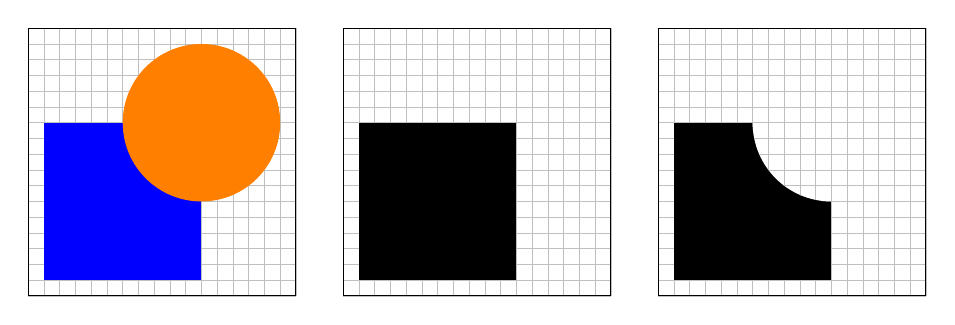
\begin{tikzpicture}
            \begin{scope}
              \draw[lightgray, very thin] (-0.2,-0.2) grid[step=0.2] (3.2,3.2);
              \fill[blue] (0,0) rectangle (2,2);
              \fill[orange] (2,2) circle (1);
              \draw[black] (-0.2,-0.2) rectangle (3.2,3.2);
            \end{scope}
            
            \begin{scope}[xshift=4cm]
              \draw[lightgray, very thin] (-0.2,-0.2) grid[step=0.2] (3.2,3.2);
              \fill[black] (0,0) rectangle (2,2);
              \draw[black] (-0.2,-0.2) rectangle (3.2,3.2);
            \end{scope}
            
            \begin{scope}[xshift=8cm]
              \draw[lightgray, very thin] (-0.2,-0.2) grid[step=0.2] (3.2,3.2);
              \fill[black] (0,0) rectangle (2,2);
              
              \begin{scope}
                \clip (0,0) rectangle (2,2);
                \clip (2,2) circle (1);
            
                \fill[white] (0,0) rectangle (2,2);
                \draw[lightgray, very thin] (-0.2,-0.2) grid[step=0.2] (3.2,3.2);
              \end{scope}
              
              \draw[black] (-0.2,-0.2) rectangle (3.2,3.2);
            \end{scope}
        \end{tikzpicture}
        
        \caption{An image with two overlapping shapes (left), the square's mask (middle), and the square's visible mask (right).}
        \label{fig:mask-visible-mask}
    \end{figure}
\end{definition}


\subsection{Bounding box}

A shape's bounding box is the smallest possible rectangle that contains the entire shape.

\begin{definition}[Bounding box]
    Given a shape 
    \[
    \gamma(t) = \left(x(t), y(t)\right)\text{,}\quad t \in \interval[scaled]{0}{1}\text{,}
    \]
    the shape's (full) bounding box is a 4-tuple 
    \[
        \left(x_{min}, y_{min}, x_{max}, y_{max}\right)\text{,}
    \]
    such that
    \begin{align}
        x_{min} &= \min_{t \in \interval[scaled]{0}{1}}{x(t)}\text{,} \\
        y_{min} &= \min_{t \in \interval[scaled]{0}{1}}{y(t)}\text{,} \\
        x_{max} &= \max_{t \in \interval[scaled]{0}{1}}{x(t)}\text{,} \\
        y_{max} &= \max_{t \in \interval[scaled]{0}{1}}{y(t)}\text{.}
    \end{align}

    Notice that by our definition, the bounding box is always \emph{axis-aligned}, meaning its sides are parallel to the axes of the Cartesian coordinate system. Such bounding boxes are also called \glspl{aabb}~\cite{smartone2024boundingboxes}. 
    
    Figure~\ref{fig:bbox} illustrates the concept of the bounding box on an example shape.

    \begin{figure}[H]
        \centering

        \begin{tikzpicture}[bezier bounding box]
            \draw[blue, ultra thick] (0,0) 
                .. controls (-1,2) and (1,3) .. (2,1)
                .. controls (3,0) and (4,4) .. (5,2)
                .. controls (6,-1) and (7,5) .. (8,3)
                .. controls (9,1) and (10,-2) .. (11,4);
                    
            \draw[dashed] (current bounding box.south west) rectangle (current bounding box.north east);
        
            \coordinate (sw) at (current bounding box.south west);
            \coordinate (se) at (current bounding box.south east);
            \coordinate (nw) at (current bounding box.north west);
            \coordinate (ne) at (current bounding box.north east);
            
            \fill (sw) circle (2pt);
            \fill (se) circle (2pt);
            \fill (nw) circle (2pt);
            \fill (ne) circle (2pt);
        
            \node[anchor=south east, xshift=1.75cm] at (nw) {$(x_{min}, y_{min})$};
            \node[anchor=south west, xshift=-1.75cm] at (ne) {$(x_{max}, y_{min})$};
            \node[anchor=north east, xshift=1.75cm] at (sw) {$(x_{min}, y_{max})$};
            \node[anchor=north west, xshift=-1.75cm] at (se) {$(x_{max}, y_{max})$};
        \end{tikzpicture}

        \caption{A composite Bézier curve (solid blue) and its bounding box (dashed black).}
        \label{fig:bbox}
    \end{figure}
\end{definition}

\begin{definition}[Visible bounding box]
    The difference between the visible bounding box and the full bounding box is analogous to the difference between the visible mask and the full mask. The visible bounding box is the bounding box of the visible parts of the element. If a part of the element is obscured by other elements, that part will not contribute to the dimensions of the visible bounding box.
\end{definition}
